\section{Análise e discussão}

\subsection{Expectativa}

\subsubsection{Hipótese 1}

Primeiramente vamos avaliar a hipótese~\ref{h:1}.
O conjunto de dados já contém a informação de que um dado componente refere-se a uma ferramenta ou não (coluna \foreign{tool} na Figura~\ref{fig:dataset}).
Assim, podemos separar o conjunto de dados em duas partes: a primeira é aquela composta pelos componentes referentes a ferramentas e a segunda, o complemento.
Existe, já há muito tempo, uma ampla discussão na literatura sobre a interpretação da escala Likert como variáveis categóricas ou se elas podem ser interpretadas como numéricas.

Aqui utilizamos as recomendações de \cite{Harpe2015}, segundo o qual escalas com mais de 5 níveis podem ser tratados como numéricos.
Esse é o caso da aprendizagem percebida.
Por isso, vamos considerar a média da aprendizagem percebida (que, sob essa suposição, pode ser calculada) em cada um dos sub-conjuntos acima, e compará-las utilizando um teste estatístico de hipótese t de \foreign{student}, variação Welch para populações com variância distinta.

Antes disso aplicamos um teste de Kolmogorov-Sinai para normalidade em cada sub-conjunto, de modo que temos certeza de que as amostras apresentam distribuição normal.
O resultado foi um valor-$p$ nulo (muito menor que o tradicional nível de significância de 5\%).
Apesar disso, segundo~\cite[p.~259]{Triola2005} é possível realizar o teste t mesmo que a amostra não apresente distribuição normal, desde que a amostra tenha tamanho maior do que 30.

\begin{figure}
	\centering
	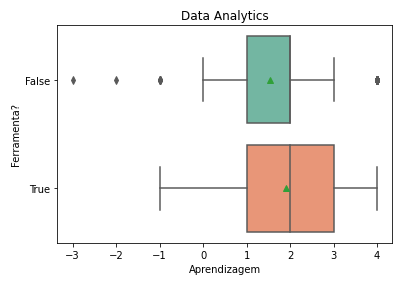
\includegraphics[width=0.45\textwidth]{da-boxplot-by-tool}\hfill
	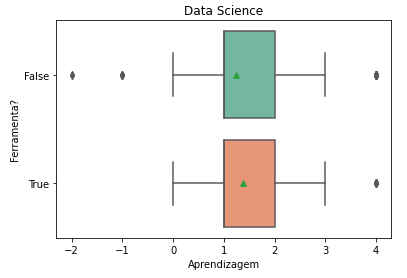
\includegraphics[width=0.45\textwidth]{ds-boxplot-by-tool}
	\caption{Boxplot dos sub-conjuntos de aulas reff. a algoritmos ou não para DA (esquerda) e DS (direita).}
\end{figure}

Vemos, então, que \emph{não} existe diferença estatisticamente significativa na aprendizagem percebida média nas aulas que envolvem ferramentas e nas que não envolvem para o curso de DS. Porém, há de fato diferença para os alunos do curso de DA.
É possível argumentar que, por sua característica voltada a técnicas de \foreign{machine learning}, ao invés de ferramentas, que é tão evidente em DA.
Essa suspeita motivou a hipótese 2, que veremos a seguir.

Á luz da teoria do valor da expectativa, é possível ainda interpretar que os alunos de DA de fato enxergam alguma vantagem nas aulas de ferramentas, possivelmente a correlação mais clara com as vagas de mercado.
Essa motivação intrínseca promove a aprendizagem do aluno naquela aula.
Uma hipótese alternativa a essa é que as aulas de ferramentas assemelham-se a tutoriais, sendo, por isso, mais simples de acompanhar, além de dar uma noção de habilidade (saber usar a ferramenta) cujo valor é mais evidente.

A aprendizagem aprimorada em ferramentas e algoritmos pode ser, alternativamente, um efeito do chamado condicionamento operante\footnote{https://www.britannica.com/topic/motivation/Behavioristic-approaches-to-motivation}. Por exemplo, a utilização das ferramentas tem como resultado algo concreto, o que pode retroalimentar a motivação do aluno. Independentemente do motivo, o fato é que há diferença. Visando aprimorar a aprendizagem nas aulas mais abstratas, pode-se procurar planejá-las também com o uso de ferramentas; aplicando-as.

Independentemente da explicação, o fato é que há diferença para DA.
Isso sugere que podemos utilizar essa motivação nas demais aulas; as mais abstratas.
Isso passa por planejar as aulas de modo que sempre fique evidente a relação com as diversas ferramentas abordadas no curso.

\begin{table}
	\caption{Tamanho das amostras, médias (e erro padrão: 95\%) e desvio-padrão de cada sub-conjunto de DA (esquera) e DS (direita).}
	\begin{minipage}{0.45\textwidth}
		\begin{tabular}{lrrr}
			\toprule
			Ferramenta? & \# & $\bar{x}$ & $s_x$ \\
			\midrule
			Sim &  365 & 0,75(1) & 0,14 \\
			Não & 1514 & 0,69(1) & 0,13 \\
			\bottomrule
		\end{tabular}
	\end{minipage}\hfill
	\begin{minipage}{0.45\textwidth}
		\begin{tabular}{lrrr}
			\toprule
			Ferramenta? & \# & $\bar{x}$ & $s_x$ \\
			\midrule
			Sim &  157 & 0,66(2) & 0,11 \\
			Não & 1606 & 0,654(5) & 0,11 \\
			\bottomrule
		\end{tabular}
	\end{minipage}
\end{table}

\begin{table}
	\centering
	\caption{Resultado do teste t nos cursos DA e DS.}
	\begin{tabular}{lcc}
	\toprule
	Curso & Valor $p$   & Estatística $t$ \\
	\midrule
	DA    & $<10^{-11}$ & $7,24$ \\
	DS    & $0,43$      & $0,78$ \\ 
	\bottomrule
	\end{tabular}
\end{table}

\subsubsection{Hipótese 2}

A verificação da hipótese 2 é similar à da primeira, exceto que dessa vez segmentamos os dados em aulas que envolvem explicitamente algoritmos e aulas mais abstratas.
Na Seção~\ref{sec:resultados} nós mostramos como essas aulas foram identificadas, restando agora executar a segmentação e o teste t.

A Tabela~\ref{tab:hipotese2-subsets} apresenta os dados dos dois sub-conjuntos de dados obtidos ao segmentar DS por algoritmo. Note que a incerteza na média da segmentação ``sim'' envolve a média da segmentação ``não''.
O desvio-padrão também é igual, mostrando que as distribuições são indistinguíveis por esses parâmetros.
Isso é evidenciado pelo teste t, que demonstra não haver diferença entre as médias.
Logo, \emph{não} temos dados suficientes para argumentar em favor da hipótese 2.
Ou seja, a presença ou não de algoritmo \emph{não} afeta a aprendizagem.

\begin{table}
	\caption{Tamanho das amostras, médias (e erro padrão: 95\%) e desvio-padrão de cada sub-conjunto de DS (direita) --- Hipótese 2.}
	\label{tab:hipotese2-subsets}
	\begin{tabular}{lrrr}
		\toprule
		Ferramenta? & \# & $\bar{x}$ & $s_x$ \\
		\midrule
		Sim &  150 &  0,67(2) & 0,11 \\
		Não & 1613 & 0,653(5) & 0,11 \\
		\bottomrule
	\end{tabular}
\end{table}

\begin{table}
	\centering
	\caption{Resultado do teste t nos cursos DA e DS.}
	\begin{tabular}{lcc}
	\toprule
	Curso & Valor $p$   & Estatística $t$ \\
	\midrule
	DS    & $0,15$      & $1,45$ \\ 
	\bottomrule
	\end{tabular}
\end{table}

\begin{figure}
	\centering
	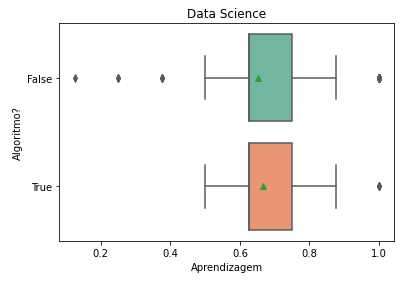
\includegraphics[width=0.45\textwidth]{ds-boxplot-by-algorithm}
	\caption{Boxplot dos sub-conjuntos de aulas reff. a algoritmos ou não para DS.}
\end{figure}

\subsubsection{Hipótese 3}

Agora voltamos nossa atenção para a possível relação entre a aprendizagem e a satisfação, ritmo e relevância reportados pelo aluno.

A teoria do valor da expectativa propõe que a motivação é uma função do produto da X por Y.
O argumento aqui é, então, que esses atributos afetam a aprendizagem.
O modelo de regressão mais simples é o linear e uma análise das correlações entre as variáveis (abaixo) de fato mostra haver correlação de Person significativa.
Porém, ao avaliar os gráficos visualmente, não é possível identificar alguma relação linear evidente, conforme podemos ver na Figura~\ref{fig:bubble-plots}.

\begin{table}
	\centering
	\caption{Métricas de qualidade dos vários modelos de regressão experimentados. $R^2$ é o índice de determinação e $\bar R^2$ é o $R^2$ ajustado à quantidade de preditores. OLR significa \foreign{ordinary least squares} (DATA SCIENCE).}
	\label{tab:reg-ds-1}
	\begin{tabular}{llccc}
		\toprule
		Modelo   & Linear? &  RMSE &   MAE & $R^2$\\
		\midrule
		XGBoost  & Não     & 0,769 & 0,581 & \textbf{0,193}\\
		\foreign{Random Forest} & Não & 0,772 & 0,594 & 0,186\\
		Árvore de decisão & Não &  0,775 & 0,596 & 0,181\\
		Adaboost & Não     & 0,806 & 0,629 & 0,113\\
		\foreign{ElasticNet} & Sim & 0,819 & 0,640 & 0,083\\
		SVR & Não & 0,835 & 0,612 & 0,048\\
		\bottomrule
	\end{tabular}
\end{table}

Então experimentamos outros algoritmos de regressão, conforme citados na Tabela~\ref{tab:reg-ds-1}.
O melhor índice de determinação obtido foi $R^2 \approx 0,193$ para o modelo XGBoost, composto por um conjunto de árvores de decisão simples\footnote{Veja, por exemplo, \url{xgboost.readthedocs.io/en/latest/tutorials/model.html}.}.
Isso significa que nosso melhor modelo é capaz de explicar apenas 19\% das variações na aprendizagem, a partir dos preditores propostos.
Embora seja baixo, podemos argumentar --- e isso pode ser vislumbrado nos gráficos --- que a aprendizagem sofre maior influência de outros parâmetros mais importantes, como a metodologia de aprendizagem, a didática do professor \etc.


Agora que sabemos que o modelos XGBoost é melhor, podemos experimentar variar os preditores.
Por exemplo, efetuamos a regressão considerando como variáveis independentes as combinações de relevância (categórica), ritmo (categõrica) e satisfação (numérica). Nesse caso, a métrica mais relevante é o $\bar R^2$, que considera a quantidade de preditores.

\begin{table}
	\centering
	\caption{$\bar R^2$ em função das possíveis combinações de variáveis independentes. O melhor modelo é aquele que tem }
	\label{tab:reg-ds-2}
	\begin{tabular}{ccccc}
		\toprule
		Relevância & Ritmo      & Satisfação & $\bar R^2$ & $R^2$\\
		\midrule
		           &            & \checkmark & \textbf{0,193} & 0,193\\
		\checkmark & \checkmark &            & 0,192          & 0,193\\
		\checkmark & \checkmark & \checkmark & 0,191          & 0,193\\
		           & \checkmark &            & 0,121          & 0,121\\
		           & \checkmark & \checkmark & 0,120          & 0,121\\
		\checkmark &            &            & 0,115          & 0,115\\
		\checkmark &            & \checkmark & 0,114          & 0,115\\
		\bottomrule
	\end{tabular}
\end{table}

Ou seja, apesar de termos três possíveis preditores, a regressão utilizando apeans a satisfação é a mais significativa, pois possui maior $\bar R^2$.
Ainda que os três primeiros modelos na Tabela~\ref{tab:reg-ds-2} apresentem o mesmo valor de $R^2$, o que significa que todos eles tem o mesmo poder de prever a aprendizagem, o fato de $\bar R^2$ ser maior para satisfação, significa que é um modelo melhor (além de ser mais simples, pois requer apenas a satisfação).



A mesma análise pode ser feita para Data Analytics

\begin{table}
	\centering
	\caption{Data Analytics}
	\label{tab:reg-da-1}
	\begin{tabular}{llccc}
		\toprule
		Modelo                  & Linear? & RMSE  &   MAE & $R^2$\\
		\midrule
		XGBoost                 & Não     & 0,958 & 0,760 & \textbf{0,213}\\
		Árvore de decisão       & Não     & 0,958 & 0,762 & 0,212\\
		\foreign{Random Forest} & Não     & 0,959 & 0,770 & 0,210\\
		Adaboost                & Não     & 0,983 & 0,801 & 0,170\\
		\foreign{ElasticNet}    & Sim     & 0,985 & 0,793 & 0,167\\
		SVR                     & Não     & 0,994 & 0,797 & 0,152\\
		\bottomrule
	\end{tabular}
\end{table}

\begin{table}
	\centering
	\caption{Data Analytics}
	\label{tab:reg-da-2}
	\begin{tabular}{ccccccc}
		\toprule
		           &            &            & \multicolumn{2}{c}{Data Science} & \multicolumn{2}{c}{Data Analytics}\\
		\midrule
		Relevância & Ritmo      & Satisfação & $\bar R^2$     & $R^2$ & $\bar R^2$     & $R^2$\\
		\midrule
		           &            & \checkmark & \textbf{0,193} & 0,193 & \textbf{0,212} & 0,213\\
		\checkmark & \checkmark &            & 0,192          & 0,193 & 0,212          & 0,213\\
		\checkmark & \checkmark & \checkmark & 0,191          & 0,193 & 0,211          & 0,213\\
		           & \checkmark &            & 0,121          & 0,121 & 0,183          & 0,184\\
		           & \checkmark & \checkmark & 0,120          & 0,121 & 0,183          & 0,184\\
		\checkmark &            &            & 0,115          & 0,115 & 0,146          & 0,147\\
		\checkmark &            & \checkmark & 0,114          & 0,115 & 0,145          & 0,147\\
		\bottomrule
	\end{tabular}
\end{table}

Note que o segundo melhor modelo, tanto para DA como DS, envolve os dois preditores complementares.
Isso sugere que satisfação é equivalente ao par relevância e ritmo.